\documentclass[12pt,a4]{article}
\usepackage[greek,english]{babel}
\usepackage{graphicx}
\graphicspath{ {./images/} }
\usepackage{hyperref}
\usepackage{xcolor}

\textwidth      6.5in
\textheight     8.7in
\oddsidemargin  0.0cm
\evensidemargin 0.0cm
\parindent      0pt
\topmargin      0.1in
\headsep        20pt

\parskip        10pt
\parindent      0pt

\newcommand{\gr}{\greektext}
\newcommand{\la}{\latintext}

\newcommand{\ilcode}[1]{\textcolor[RGB]{160, 110, 220}{#1}}

\begin{document}

\begin{titlepage}
	\begin{center}
		% Title.
		\vspace*{1cm}
		\Huge
		\textbf{{\la Intro to Git}}
		
		% Subtitle.
		\vspace{0.5cm}
		\LARGE
		{\sf \la Workshop}

		% Participants in alphabetical order.
		\vspace{1.5cm}
		\normalsize
		\textbf{Κιορπελίδης Πλάτων}\\
		\textbf{Μπαζιότης Στέφανος}

		\vfill
		
		%\includegraphics[width=0.4\textwidth]{uni-logo}
		\scalebox{2}{%
			
\includegraphics[width=0.4\textwidth]{acmuoa}}

		\LARGE
		{\sf \la University of Athens}\\
		{\sf \la ACM UoA Student Chapter}

		% Some cool coffee stains.
		\cofeAm{0.08}{0.8}{120}{200}{-200}
		\cofeAm{0.06}{0.8}{240}{150}{-140}
	\end{center}
\end{titlepage}


\section{Introduction}
\subsection{Git \& Version Control}
{\sf -- \emph{The Problem}:}
Many people’s version-control method of choice is to copy files into another
directory. We create copies of the project and name them to \emph{project v2},
\emph{project v3}, etc. This approach is very common because it is so simple,
but it is also incredibly error prone. It is easy to forget which directory
you’re in and accidentally write to the wrong file or copy over files you don’t
mean to, delete code that may be useful later -- whenever you have the entire
history of the project in a single place, you risk losing everything. In
addition, it clutters up the workspace and gives vertigo to anyone browsing it.

We also want to collaborate with other developers. We could keep the codebase
under a server but what about server failures. If the server goes down for an
hour, then during that hour nobody can collaborate at all or save versioned
changes to anything they're working on. If the hard disk the central database is
on becomes corrupted, and proper backups haven’t been kept, you lose absolutely
everything -- the entire history of the project except whatever single snapshots
people happen to have on their local machines.

{\sf -- \emph{The Solution}:} This is where Distributed Version Control Systems
step in, like Git. In such systems, clients don’t just check out the latest
snapshot of the files; rather, they fully mirror the repository, including its
full history. Thus, if any server dies, and these systems were collaborating via
that server, any of the client repositories can be copied back up to the server
to restore it. Every clone is really a full backup of all the data.

\textcolor[RGB]{220,220,220}{\rule{\linewidth}{0.8pt}}

{\sf Version Control:} It's is a system that records changes to a file or a set
of files over time so that you can recall specific versions later.

{\sf Distributed Version Control System:} Clients fully mirror the remote
repository, including it's history. Remote repository is stored in a server.
Full copy of the code is present in all the developers' computers.

Popularity of Git (2010 vs 2019):
\vspace*{-5pt}
\begin{itemize}
\item 2010: 26,485 repositories (11.3\% of total)
\item 2019: 913,378 repositories (70\% of total)
\end{itemize}

{\sf Server example:} GitHub. GitHub is the single largest hosting server for
Git repositories with a web front end. It offers all of the distributed version
control and source code management (SCM) functionality of Git as well as adding
its own features. It provides access control (users) and several collaboration
features such as bug tracking, feature requests, task management, and wikis for
every project. A large percentage of all Git repositories are hosted on GitHub,
and many open-source projects use it for Git hosting, issue tracking, code
review, and other things. So while it’s not a direct part of the Git open source
project, there’s a good chance that you’ll want or need to interact with GitHub
at some point while using Git professionally.

\subsection{Concept of Git \& Early days}
Git follows the unix philosophy. The Unix philosophy emphasizes building simple,
short, clear, modular, and extensible code that can be easily maintained and
repurposed by developers other than its creators. The Unix philosophy favors
composability as opposed to monolithic design.

In it's early days git consisted of simple, atomic executables. Such programs
weren't enough to be useful on their own, but a combination of those, usually in
shell scripts, composed more complex functionality like \ilcode{\bf git add}.
Probably it's the reason, after so many developement cycles, still considered a
complex and difficult tool.

It was created by Linus Torvalds to help maintain Linux. As more people were
sending in patches and the current workflow didn't scale, Linus created a new
VCS as he didn't like existing ones. He named it git -- the stupid content
tracker or the information manager from hell.

\subsection{Modern Git}
Initially git wasn't developed for the novice user. Nowdays it's a lot
friendlier and easier to get into as it comes with a lot of build-in commands,
wrappers and complexity abstractions. These commands internally use the old,
enhanced, but still atomic executables. There are GUIs developed for the GUI
lovers or non-technical people and it's supported with plugins by various text
editors and IDEs. These changes and features make for an easier, faster and
streamlined collaboration between developers, who follow various local and
online workflows.

\subsection{Meaning of Git}
\vspace*{-10pt}
\emph{Copied from the first git commit written by Linus Torvalds.}

"git" can mean anything, depending on your mood.
\begin{itemize}
\vspace*{-10pt}
\item Random three-letter combination that is pronounceable, and not actually
	used by any common UNIX command. The fact that it is a mispronounciation of
	"get" may or may not be relevant.
\vspace*{-3pt}
\item Stupid. Contemptible and despicable. Simple. Take your pick from the
	dictionary of slang.
\vspace*{-3pt}
\item "global information tracker": you're in a good mood, and it actually
   works for you. Angels sing, and a light suddenly fills the room.
\vspace*{-3pt}
\item "goddamn idiotic truckload of sh*t": when it breaks.
\vspace*{-10pt}
\end{itemize}

This is a stupid (but extremely fast) directory content manager. It doesn't do
a whole lot, but what it does do is track directory contents efficiently.

\section{Installing Git}
Before you start using Git, you have to make it available on your computer. Even
if it’s already installed, it’s probably a good idea to update to the latest
version. You can either install it as a package or via another installer, or
download the source code and compile it yourself.

{\sf -- Linux (Debian, Ubuntu):} \ilcode{sudo apt-get install git-all}

{\sf -- Mac:} Run \ilcode{git -{}-version}. If you don’t have it installed
already, it will prompt you to install.

{\sf -- Windows:} Download from \url{https://git-scm.com/download/win}.

\section{Working locally}
\subsection{Initializing Git (git init)}
If you have a project directory that is currently not under version control and
you want to start controlling it with Git, you first need to go to that
project’s directory \ilcode{cd /home/user/my\_project} and type \ilcode{git
init}. This creates a new subdirectory named .git that contains all of your
necessary repository files -- a Git repository skeleton. A project that is under
Git is called "repository" or "repo". At this point, nothing in your project is
tracked yet.

In order to start tracking our changes and as a result our project we need to
inform Git about our identity. This is important because every Git commit uses
this information, and it’s immutably baked into the commits you start creating:

\hspace*{1cm}
\ilcode{\$ git config --global user.name "John Doe"}\\
\hspace*{1cm}
\ilcode{\$ git config --global user.email johndoe@example.com}

{\sf NOTE:} \ilcode{-{}- global} sets your name and email across Git projects.
If you want to have a different identity for different projects run the above
instructions without \ilcode{-{}- global} flag. You can check your settings with
\ilcode{git config -{}- list}.

\begin{center}
\scalebox{2}{%
	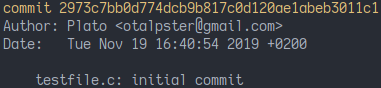
\includegraphics[width=0.4\textwidth]{gitlog}}
\end{center}

{\sf -- \emph{Exercise}:} Open your laptops! Open a terminal and create a
directory. Inside the new directory run \ilcode{git init}. Then run \ilcode{ls
-la} and notice the hidden directory \ilcode{.git}.

\subsection{The three stages}
\begin{center}
\scalebox{2.5}{%
	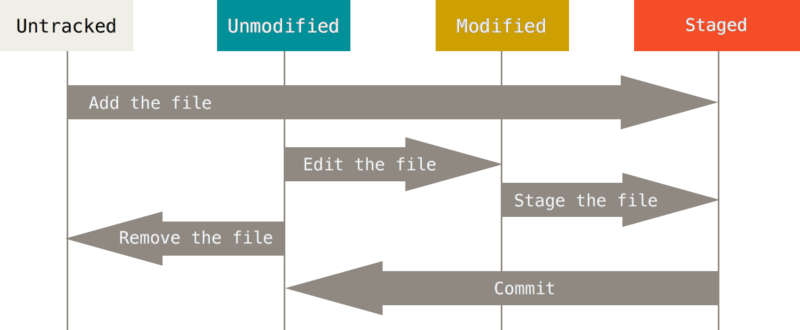
\includegraphics[width=0.4\textwidth]{lifecycle}}
\end{center}

Each file in your working directory can be in one of two states: tracked or
untracked. Tracked files are files that were in the last snapshot; they can be
unmodified, modified, or staged. In short, tracked files are files that Git
knows about.

Untracked files are everything else -- any files in your working directory that
were not in your last snapshot and are not in your staging area. When you first
create a file it will be untracked because Git does not track it yet.

As you edit files, Git sees them as modified, because you’ve changed them since
your last commit. As you work, you selectively stage these modified files and
then commit all those staged changes, and the cycle repeats.

\subsection{Checking the status of your file (git status)}
The tool you use to determine which files are in which state is the \ilcode{git
status} command.

{\sf -- \emph{Exercise}:} Run \ilcode{git status}. Create a new file
\ilcode{touch testfile}. Run \ilcode{git status} again. The new file should
appear as \ilcode{untracked}.

\subsection{Staging changes (git add)}
\ilcode{git add} moves changes to the staging area. Changes to Git means
anything it does not know, new files or modified ones. The staging area is where
we are cooking the contents of our next snapshot.

{\sf -- \emph{Exercise}:} Let's track our new file. Run \ilcode{git add}. See
that our new file is in the staging area with \ilcode{git status}. Now our
untracked file is cooking for the next snapshot! When Git records the current
staging area and creates a new snapshot our untracked file will become tracked.
Until then it's just staged.

{\sf -- \emph{Exercise}:} Open your editor of choice and change the testfile.
Add some random letters. Run \ilcode{git status}. Notice that the testfile is
listed as both staged and unstaged.

How is this possible? It turns out that Git stages a file exactly as it is when
you run \ilcode{git add}. If you record a new snapshot now, the version of
testfile as it was when you last ran \ilcode{git add} is how it will go into the
snapshot, not the version of the file as it looks in your working directory. If
you modify a file after you run \ilcode{git add}, you have to run \ilcode{git
add} again to stage the latest version of the file.

\subsection{Viewing your staged and unstaged changes (git diff)}
Sometimes, \ilcode{git status} command is too vague. You want to know exactly
what you changed, not just which files were changed. To achive this you use the
\ilcode{git diff} command. You most often use it to answer these two questions:
What have you changed but not yet staged? What have you staged that you are
about to commit? \ilcode{git status} answer these questions by listing the file
names, \ilcode{git diff} shows you the exact lines added and removed -- the
patch, as it were.

To see changes you've made that you haven't yet staged, type \ilcode{git diff}.
That command compares what is in your working directory with what is in your
staging area.

To see what you’ve staged that will go into your next commit, you can use
\ilcode{git diff -{}-staged}. This command compares your staged changes to your
last commit.

{\sf -- \emph{Exercise}:} View your changes. Run \ilcode{git diff}. Run
\ilcode{git diff -{}-cached}. Notice the + and - characters. What do they mean?
+, - describes the added and removed lines respectively.

It’s important to note that \ilcode{git diff} by itself doesn’t show all changes
made since your last commit -- only changes that are still unstaged. If you’ve
staged all of your changes, \ilcode{git diff} will give you no output. You will
need to run \ilcode{git diff} and \ilcode{git diff -{}-staged} to show all changes
made since your last commit, staged and unstaged.

\ilcode{git status} can reproduce the above behaviour by running internally and
formatting the output of \ilcode{git diff} and \ilcode{git diff -{}-staged} with
the flag \ilcode{git status -v}/\ilcode{-vv}. The \ilcode{-v} flag, in addition
to the output of \ilcode{git status}, will also show the actual changes that are
staged to be committed, like \ilcode{git diff -{}-cached}. The \ilcode{-vv}
flag, in addition to the output of \ilcode{git status -v}, will also show the
changes that have not yet been staged, like \ilcode{git diff}.

{\sf -- \emph{Exercise}:} View your changes. But this time run \ilcode{git
status -v}. Run \ilcode{git status -vv}. See the difference and the similarity
with \ilcode{git diff}/\ilcode{git diff -{}-cached}?

\subsection{Snapshoting/Committing your changes (git commit)}
Now that your staging area is set up the way you want it, you can commit your
changes. Remember that anything that is still unstaged -- any files you have
created or modified that you haven’t run \ilcode{git add} on since you edited
them -- won’t go into this commit. They will stay as modified files on your
disk. So you’re ready to commit your changes. The simplest way to commit is to
type \ilcode{git commit}.

Each commit consists of the {\bf commit message} and a {\bf body}. It's a common
practise to write commit messages with up to 50 characters. Commit messages are
used for a brief but descriptive explanation about what changes you are
committing. The body should provide a meaningful commit message, for example:
\begin{itemize}
\item Explains the problem the change tries to solve, i.e. what is wrong with
	the current code without the change.
\item Justifies the way the change solves the problem, i.e. why the result with
	the change is better.
\item Alternate solutions considered but discarded, if any.
\end{itemize}
If your description starts to get too long, that’s a sign that you probably need
to split up your commit to finer grained pieces. Descriptions that summarize the
point in the subject well, and describe the motivation for the change, the
approach taken by the change, and if relevant how this differs substantially
from the prior version, are all good things to have.

{\sf -- \emph{Exercise}:} Commit your changes. Run \ilcode{git commit}. Doing so
will launch the default editor with the output of \ilcode{git status} commented
out. The first line is the commit message. Leave a blank line and write a short
description.

{\sf -- \emph{Exercise}:} Stage your changes. Run \ilcode{git add}. Now commit
them. Sometimes you forget what you are committing and need even more explicit
reminder than the commented out \ilcode{git status}. Run \ilcode{git commit -v}.
Doing so also puts the diff of your change in the editor so you can see exactly
what changes you're committing. Save and exit the editor to create your commit.

Alternatively, you can type your commit message inline with the commit command
by specifying it after a -m flag, like this:

\hspace*{1cm}
\ilcode{\$ git commit -m "Story 182: Fix benchmarks for speed"}

Remember that the commit records the snapshot you set up in your staging area.
Anything you didn’t stage is still sitting there modified; you can do another
commit to add it to your history. Every time you perform a commit, you’re
recording a snapshot of your project that you can revert to or compare to later.

\subsection{Viewing the commit history (git log)}
After you have created several commits, or if you collaborate with others and
they made changes (more later), you’ll probably want to look back to see what
has happened. The most basic and powerful tool to do this is the \ilcode{git
log} command.

By default, with no arguments, \ilcode{git log} lists the commits made in that
repository in reverse chronological order; that is, the most recent commits show
up first. As you can see, this command lists each commit with its SHA-1
checksum, the author’s name and email, the date written, and the commit message.

A huge number and variety of options to the git log command are available to
show you exactly what you’re looking for. Here, we’ll show you some of the most
useful.

{\sf -- \emph{Exercise}:} Run \ilcode{git log -{}-one-line}. One line per commit.

{\sf -- \emph{Exercise}:} Run \ilcode{git log -n}. Show the last $n$ commits.

{\sf -- \emph{Exercise}:} Run \ilcode{git log -p}. Show the changes introduced.

{\sf -- \emph{Exercise}:} Run \ilcode{git log -{}-stat}. Abbreviated commit stats.

\subsection{Undoing staged and modified changes}
At any stage, you may want to undo something. Here, we’ll review a few basic
tools for undoing changes that you’ve made. Be careful, because you can’t always
undo some of these undos. This is one of the few areas in Git where you may lose
some work if you do it wrong.

\subsubsection{Unstaging a Staged File}
You made a mistake and ran \ilcode{git add} against a file which you don't want
to commit yet. How can you unstage it? The \ilcode{git status} command reminds
you.

{\sf -- \emph{Exercise}:} Make a very simple change. Run \ilcode{git add}. Now
run \ilcode{git status}. Run \ilcode{git reset HEAD testfile} to unstage. The
command is a bit strange, but it works. The testfile file is modified but once
again unstaged.

{\sf NOTE:} \ilcode{git reset} can be a dangerous command. However, in the
scenario described above, the file in your working directory wasn't touched, so
it’s relatively safe.

\subsubsection{Unmodifying a Modified File}
What if you realize that you don’t want to keep the changes you made to a file?
How can you easily unmodify it -- revert it back to what it looked like when you
last committed? Luckily, \ilcode{git status} tells you how to do that, too.

{\sf -- \emph{Exercise}:} Run \ilcode{git status}. Run \ilcode{git checkout
-{}- testfile}. You can see that the changes have been reverted.

{\sf NOTE:} It’s important to understand that \ilcode{git checkout -{}-
$<$file$>$} is a dangerous command. Any local changes you made to that file are
gone -- Git just replaced that file with the most recently-committed version.
Don’t ever use this command unless you absolutely know that you don’t want those
unsaved local changes.

Know that anything that is committed in Git can almost always be recovered. Even
commits that were deleted or commits that were overwritten/modified can be
recovered. However, anything you lose that was never committed is likely never
to be seen again.

\subsection{Branching}
Branching means you diverge from the main line of development and continue to do
work without messing with that main line. Sometimes you want to experiment with
an idea, implement a new feature or fix a bug, in a seperate "container",
without messing or changing the main line, stable "master" branch, making it
unstable -- with unfinished, bug-ridden -- work in progress changes. Maybe you
were working on a new feature and an critical bug needs to be fixed immediately.
You need to somehow save your work and fix that bug.

\begin{center}
\scalebox{2}{%
	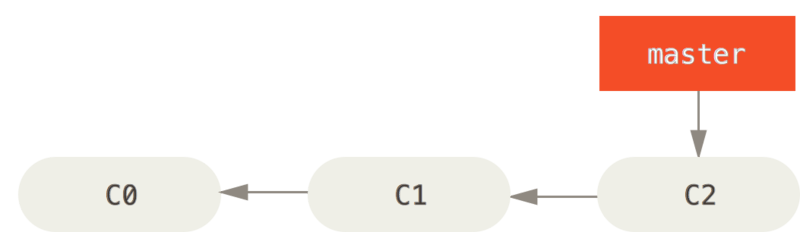
\includegraphics[width=0.4\textwidth]{basic-branching-1}}
\end{center}

A branch is simply a movable pointer to a commit. The default branch name in Git
is master. As you start making commits, you’re given a master branch that points
to the last commit you made. Every time you commit, the master branch pointer
moves forward automatically.

The \"master\" branch in Git is not a special branch. It is exactly like any
other branch. The only reason nearly every repository has one is that the
\ilcode{git init} command creates it by default and most people don’t bother to
change it.

Git encourages workflows that branch and merge often, even multiple times in a
day. Understanding and mastering this feature gives you a powerful and unique
tool and can entirely change the way that you develop.

{\sf -- \emph{Exercise}:} List the existing branches. Run \ilcode{git branch}.
Notice that only master exists.

\subsubsection{Create a branch}

\begin{center}
\scalebox{2}{%
	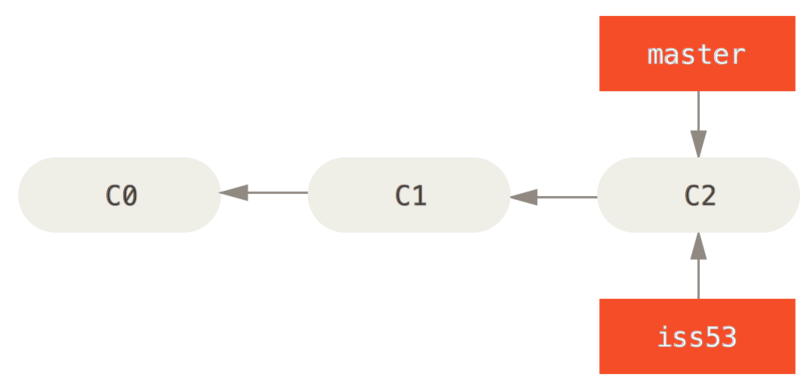
\includegraphics[width=0.4\textwidth]{basic-branching-2}}
\end{center}

Let's create a new branch. Creating a branch "testbranch" means we create a
new pointer, named "testbranch" for us to move around.

{\sf -- \emph{Exercise}:} Create a new branch. Run \ilcode{git branch
testbranch}. This creates a new pointer to the same commit you’re currently on.
\ilcode{git branch} only created a new branch -- it didn’t switch to that
branch. Run \ilcode{git branch} again. Notice the new branch and the branch you
are on which is indicated by the asterisk.

{\sf -- \emph{Exercise}:} Where are the branch pointers pointing? Run
\ilcode{git log}. You can see the "master" and "testing" branches that are right
there next to the last commit.

\subsubsection{Working on branches and diverging history}

Let's switch to our new branch and make a change. To switch to an existing
branch, you run the \ilcode{git checkout} command.

{\sf -- \emph{Exercise}:} Switch to the new branch. Run \ilcode{git checkout
testbranch}. Run \ilcode{git branch}. Notice the asterisk is next to testbranch
now.

{\sf -- \emph{Exercise}:} Open the testfile file and make a tiny change. Run
\ilcode{git status} and verify the file indeed changed. You may want to see the
actual changes in which case run \ilcode{git diff}. Stage the changes with
\ilcode{git add} and commit them with \ilcode{git commit -m "Tiny change"}. You
can pick any commit message you think is correct. Run \ilcode{git log} and
notice that testbranch moved forward and master did not.

Let's change to master branch and also make a change there.

{\sf -- \emph{Exercise}:} Change back to master branch. Run \ilcode{git checkout
master}.

Notice the files in your working directory reverted back to the snapshot that
master branch points to. If Git cannot do it cleanly (you have uncommitted
changes that conflict), it will not let you switch at all. This also means the
changes you make from this point forward will diverge from an older version of
the project. It essentially rewinds the work you've done in your testbranch
branch so you can go in a different direction.

{\sf -- \emph{Exercise}:} Change testfile file. Run \ilcode{git add} and
\ilcode{git commit -m}.

Now your project history has diverged. You created and switched to a branch, did
some work on it, and then switched back to master branch and did other work.
Both of those changes are isolated in separate branches. You can switch back and
forth between the branches.

{\sf -- \emph{Exercise}:} We can easily see the diverged history with
\ilcode{git log}. Run \ilcode{git log -{}-oneline -{}-graph -{}-all}.

\begin{center}
\scalebox{2.5}{%
	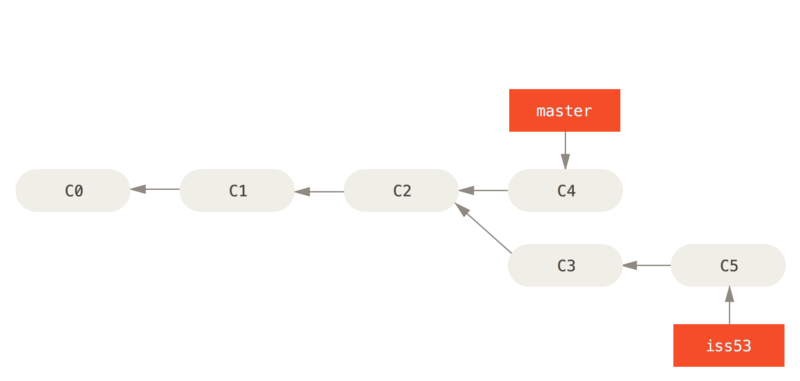
\includegraphics[width=0.4\textwidth]{basic-branching-6}}
\end{center}

\subsubsection{Merging branches}
You finished a piece of work, tested it and you want to merge/unify it back into
the main line of development. You can do that using \ilcode{git merge}. Let's do
it.

{\sf -- \emph{Exercise}:} Switch to the branch you want to merge your feature
in. In our example we are already in master branch and we want to merge
testbranch. Run \ilcode{git merge testbranch}.

Git has various algorithms/strategies to merge branches together. \ilcode{git
merge} will automatically select a merge strategy unless explicitly specified.
There are explicit and implicit merges. We will cover fast-forward and recursive
methods. Fast-forward is an implicit merge. We can perform a fast-forward merge
if the branch we are merging into has not diverged. In such case Git simplifies
things by moving the pointer forward because there is no divergent work to merge
together. Recursive merge on the other hand is an explicit merge. The explicit
part is that they create a new \"merge\" commit. Recursive is the default merge
strategy when merging one branch. Git will attempt to find a common ancestor
between the two branches. Once git finds a common ancestor it will create a new
\"merge commit\" that combines the changes of the two branches. Technically, a
merge commit is a regular commit which just happens to have two parent commits.

In this case, your development history has diverged from some older point.
Because the commit on the branch you’re on isn’t a direct ancestor of the branch
you’re merging in, Git has to do some work as it cannot fast-forward.

Occasionally, this process doesn’t go smoothly. If you changed the same part of
the same file differently in the two branches you’re merging, Git won’t be able
to merge them cleanly. If your change in branch master modified the same part of
a file as the testbranch branch, you’ll get a merge conflict. In other cases, If
you didn't change the same part of the file or the branch you are merging into
does not have any changes after you branched out, it will merge cleanly.

\begin{center}
\scalebox{2.5}{%
	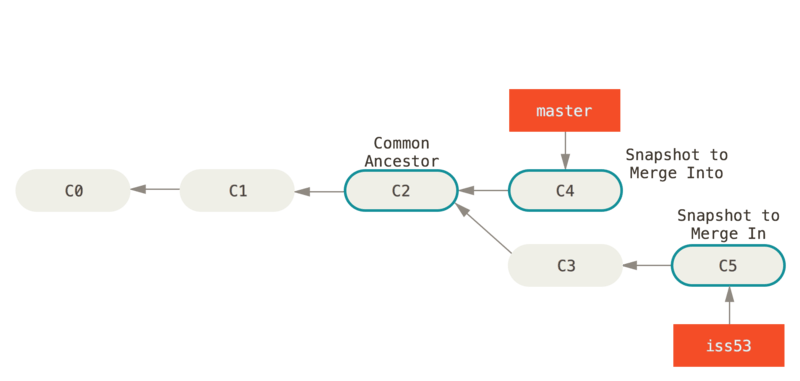
\includegraphics[width=0.4\textwidth]{basic-merging-1}}
\end{center}

Anything that has merge conflicts and hasn’t been resolved is listed as
unmerged. Git adds standard conflict-resolution markers to the files that have
conflicts, so you can open them manually and resolve those conflicts. Merge
conflicts appear with a block that contains \ilcode{$<<<<<<<$}, \ilcode{=======}
and \ilcode{$>>>>>>>$}. The top part of that block, everything above
\ilcode{=======}, is the branch you are merging into and everything bellow is
the branch you are merging in. In order to resolve the conflict, you have to
either choose one side or the other or merge the contents yourself. After you’ve
resolved each of these sections in each conflicted file, run \ilcode{git add} on
each file to mark it as resolved. Staging the file marks it as resolved in Git.

At this point, after running \ilcode{git merge} you should have a merge
conflict. Changes from the testbranch conflict with changes from master branch.
Git hasn’t automatically created a new merge commit. It has paused the process
while you resolve the conflict. If you want to see which files are unmerged at
any point after a merge conflict, you can run \ilcode{git status}.

{\sf -- \emph{Exercise}:} Open testfile file and resolve the conflict. Notice
the conflict block with the markers. Solve the conflict and stage the file.
Create the merge commit with \ilcode{git commit}.

If you think it would be helpful to others looking at this merge in the future,
you can modify this commit message with details about how you resolved the merge
and explain why you did the changes you made if these are not obvious.

\begin{center}
\scalebox{2.5}{%
	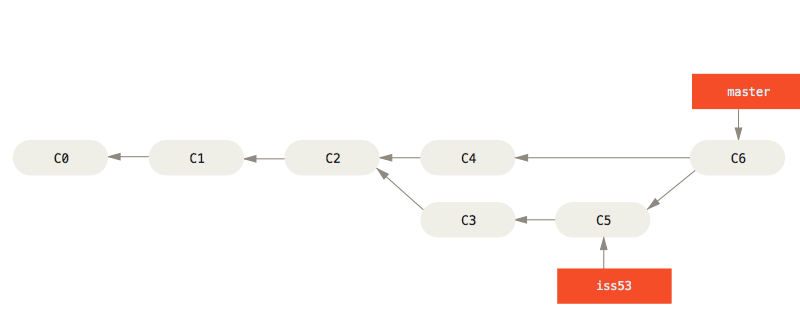
\includegraphics[width=0.4\textwidth]{basic-merging-2}}
\end{center}

\subsubsection{Deleting branches}
After you implement or fix a bug you no have no further need for the branch. You
can delete it with \ilcode{git branch -d $<$branchname$>$}. This command deletes
branches that have been merged into the branch you are currently in. If the
branch you are trying to delete contains work that isn't merged in yet, trying
to delete it will fail. If you really want to delete such branch and lose that
work, you can force it with \ilcode{-D} flag, \ilcode{git branch -D
$<$branchname$>$}.

{\sf -- \emph{Exercise}:} Delete branch testbranch. Run \ilcode{git branch -d
testbranch}. Run \ilcode{git branch} and notice the branch no longer exists.
\end{document}
